% status: 100
% chapter: Benford's Law Verification

\title{Universal Cloud REST Service Framework to Determine 
 the Validity Of Benford’s Law Using Datasets In Data.gov}

\author{Ravinder Lambadi}
\affiliation{%
  \department{School of Informatics, Computing, and Engineering}
  \institution{Indiana University}
  \city{Bloomington}
  \state{IN}
  \postcode{47408}
  \country{USA}}
\email{rlambadi@iu.edu}


\author{Orly Esteban}
\affiliation{%
  \department{School of Informatics, Computing, and Engineering}
  \institution{Indiana University}
  \city{Bloomington}
  \state{IN}
  \postcode{47408}
  \country{USA}}
\email{esteban@iu.edu}

\begin{abstract}
It is observed that a lot of real-life data, from personal 
expenses to world population data, tend to obey Benford’s Law. 
Because of this phenomenon, Benford’s Law has been leveraged 
in a lot of statistical analysis – including fraud detection. 
In 2009,  Benford’s Law has been utilized to detect election 
fraud in Iran. In this paper, the authors will determine the 
universality of the law. Is the law applicable to any dataset? 
The authors will analyze and visualize data on publicly 
available data sets at data.gov and determine which 
datasets follow this law and which ones do not, if any.

In this paper, the authors created web services deployed 
on the cloud that take large datasets, analyze them and 
return a graph that shows the leading digits distribution 
of the selected field in the dataset compared side by side 
with Benford’s Law predicted distribution.

\end{abstract}

\keywords{hid-sp18-514, hid-sp18-506, REST, Benford's Law, Python}

\maketitle

\section{Introduction}
Benford’s law is a phenomenon about the distribution 
of the first-digits of numerical sets of real-life data. 
The law states that the distribution of the first digits
follows a certain mathematical pattern. If the probability 
distribution of the digits is evenly flat, each digit from 
1 thru 9 would appear 11 percent of the time. However, 
with with Bendford’s Law, The probability distribution 
tends to go lower from the digit 1 to the digit 
9~\cite{hid-sp18-514-benfordwiki}.
For example, the digit 1 tends to occur about 30 percentage 
of the time while the digit 9 about 4.6 percentage 
of the time. The chart below shows the frequency of 
leading digits that obey Benford’s Law vs flat even distribution


\begin{figure}[!ht]
\centering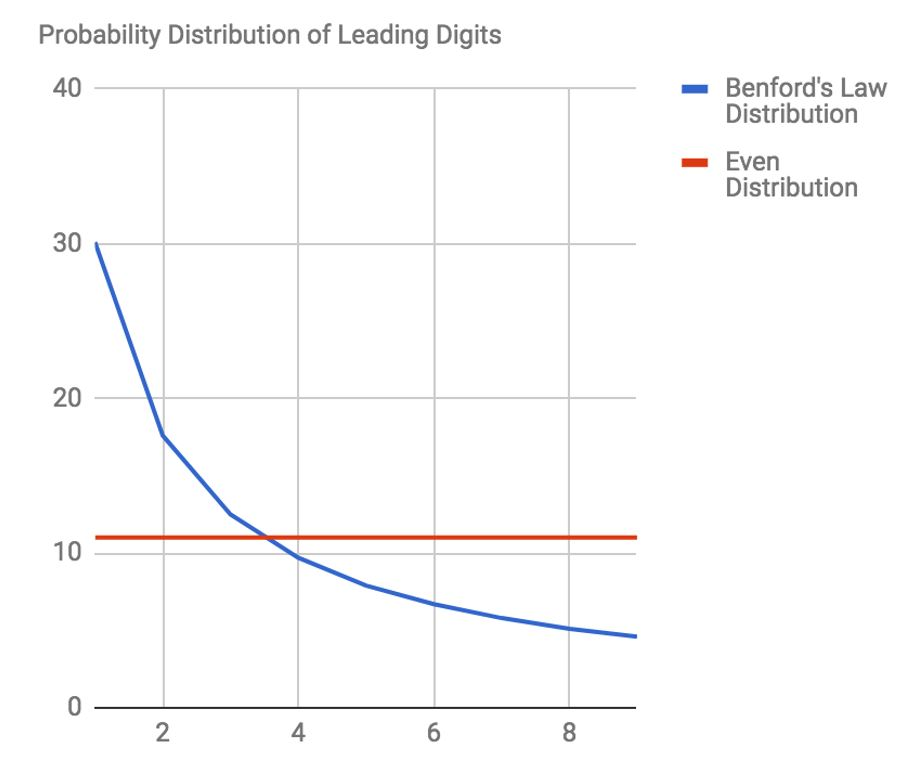
\includegraphics[width=\columnwidth]{images/probability_dist.JPG}
  \caption{Probability distribution of Leading Digits}\label{f:prob-dist-lead}
\end{figure}

Because of this phenomena, Benford’s Law is used in many 
fraud detection algorithms. The Bureau of Internal Revenue 
Service uses this law to catch tax cheats. 
A presidential election fraud was detected in 
Iran in 2009 thru the application of Benford’s Law.


A dataset is said to satisfy Benfords Law if the leading 
digits have the following the probability distribution: 

\begin{figure}[!ht]
\centering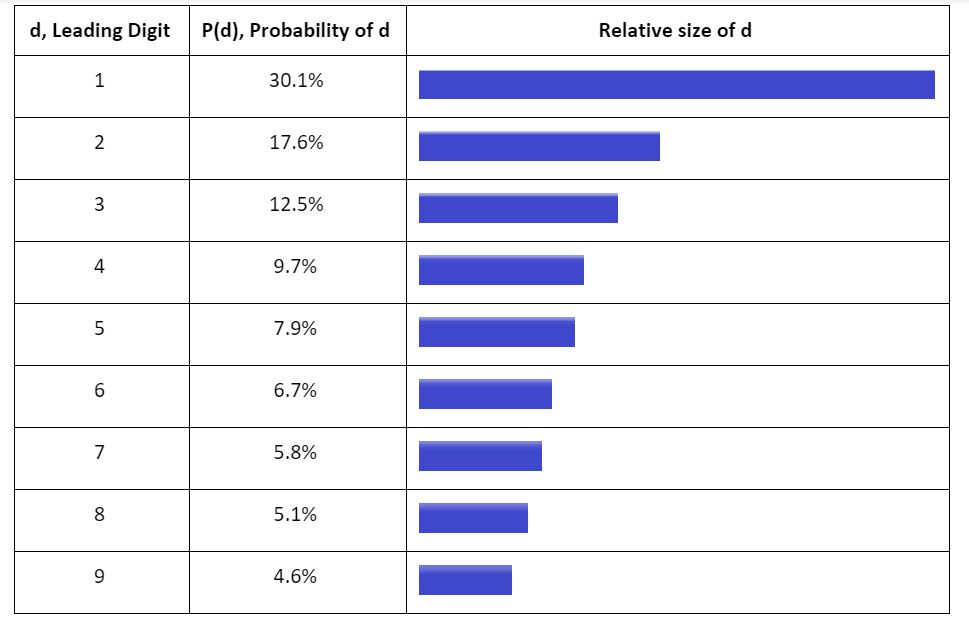
\includegraphics[width=\columnwidth]{images/benfords_law.JPG}
  \caption{Probability distribution of Benfords Law}\label{f:prob-dist-ben}
\end{figure}


In mathematical terms, Benford’s Law can be represented 
by the following equation:

P (d) = log (d+1) - log (d)

Example: In case base 10 is used we obtain the 
probability for the leading digit 1, as

P (1) = log (1+1) - log (1) = 0.301

which means, if the dataset complies 
with Benford's Law, the probability of finding a 
leading digit 1 is about 30.1 percentage of the time. 
Therefore, Benford’s Law indicates that the most 
likely leading digit for us to see is 1, the second 
most likely 2, the third most 3, the fourth most 
likely 4, and so on.

Some real-life examples of data where Benford’s Law is 
seen in the choice of iPhone passcodes. 
It is determined that most passcodes start with a 1 or  
2 and least with a 9. The yellow bars show the actual
distribution compared to the Benford’s 
Law expected distribution indicated by the 
red triangles~\cite{hid-sp18-514-iphone-benford}

\begin{figure}[!ht]
\centering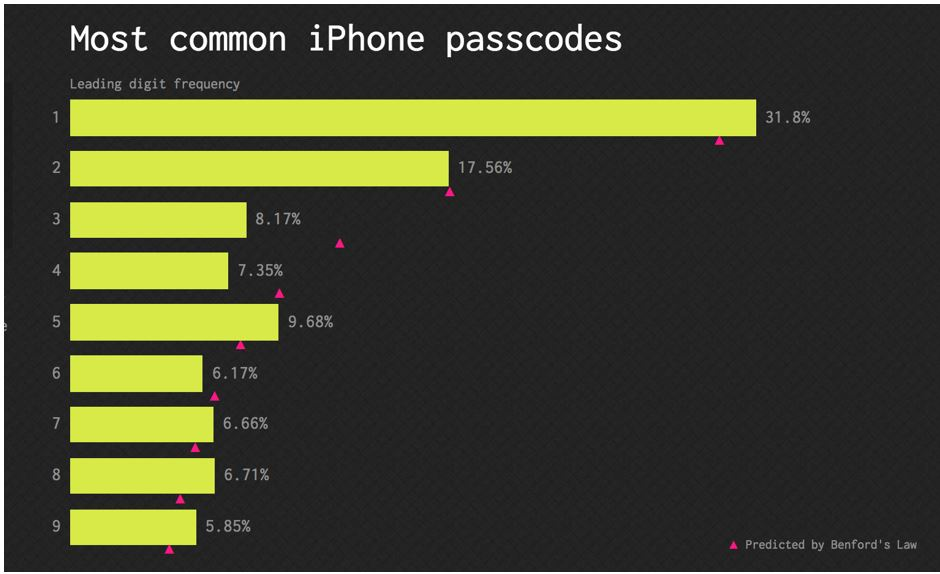
\includegraphics[width=\columnwidth]{images/iphone_benford.JPG}
  \caption{Testing Benford's Law for iPhone Passcodes}\label{f:iphone-pass_ben}
\end{figure}


Another example is the distribution of the first 
digits of the population of more than 200 countries 
in the world as shown in the graph below. 
The red bars show the distribution while 
the black dots show the distribution as 
predicted by Benford’s Law~\cite{hid-sp18-514-benfordwiki}

\begin{figure}[!ht]
\centering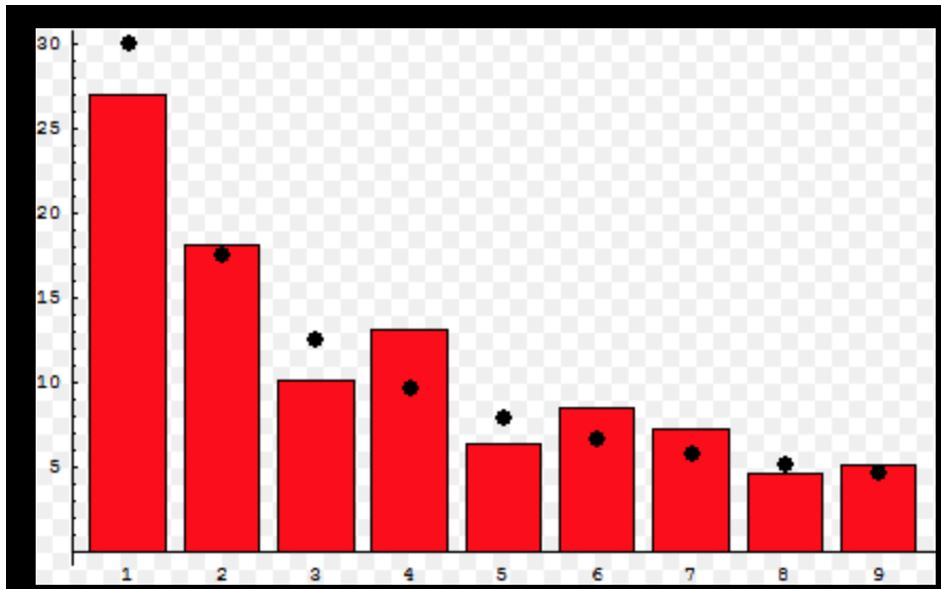
\includegraphics[width=\columnwidth]{images/benford_country.JPG}
  \caption{First Digit Population Distribution}\label{f:pop-dist-countries}
\end{figure}

\section{REST Services To Determive Benfords's Law}

There are four universal services have been built to determine
whether the provided data set follows Befords's law.

\begin{enumerate}
 \item downloadDataSet
 \item computeBenfordLawCSVDataSet
 \item computeBenfordLawExcelDataSet
 \item computeBenfordLawWebDataSetService
\end{enumerate}


\subsection{downloadDataSet}
downloadDataSet is a REST API service tested on 
on-premise and cloud environment. This service requires two 
input paramaters to download the dataset.

Below parameters need to pass to this REST API:

\begin{enumerate}
\item dataLocation - Location of the dataset. 
 Ex:~\cite{hid-sp18-514-excelDatalocation}
\item fileName - Dataset file name to be downloaded 
 as, Ex: nsn-extract.xlsx
\end{enumerate}


\subsection{computeBenfordLawExcelDataSet}
computeBenfordLawExcelDataSet is a REST API service tested on 
on-premise and cloud environment. This service requires two 
input paramaters to determine Befords's Law. This service
process and send back the output 
for all excel based datasets.

Below parameters need to pass to this REST API:

\begin{enumerate}
\item columnName - Name of the column in the 
 dataset for which Benford Law determation required. 
 Ex: Price
\item fileName - Dataset file name to be downloaded 
 as, Ex: nsn-extract.xlsx
\end{enumerate}

\subsection{computeBenfordLawCSVDataSet}
computeBenfordLawCSVDataSet is a REST API service 
tested on on premise and cloud environment. 
This service requires two input paramaters to 
determine Befords's Law. This service
process and send back the output 
for all CSV and Text based datasets.

Below parameters need to pass to this REST API:

\begin{enumerate}
\item columnName - Name of the column in the 
 dataset for which Benford Law determation required. 
 Ex: COUNT PUBLIC ASSISTANCE TOTAL
\item fileName - Dataset file name to be downloaded 
 as,Ex: DemographicStatistics.csv
\end{enumerate}

\subsection{Benfords Law Verification for National Stock 
Number Extract Datset - Excel}
National Stock Number extract includes the current 
listing of National Stock Numbers, 
NSN item name and descriptions, and current 
selling price of each product listed in GSA 
Advantage and managed by GSA. Each NSN is 
listed with the vendors description of the item. 
Some descriptions exceed the standard length and are 
truncated~\cite{hid-sp18-514-nsn-ds-desc}.

BenfordLawExcelDataSetService returned the below
output for the dataset~\cite{hid-sp18-514-excelDatalocation}
and columns name was:Price.

\begin{figure}[!ht]
\centering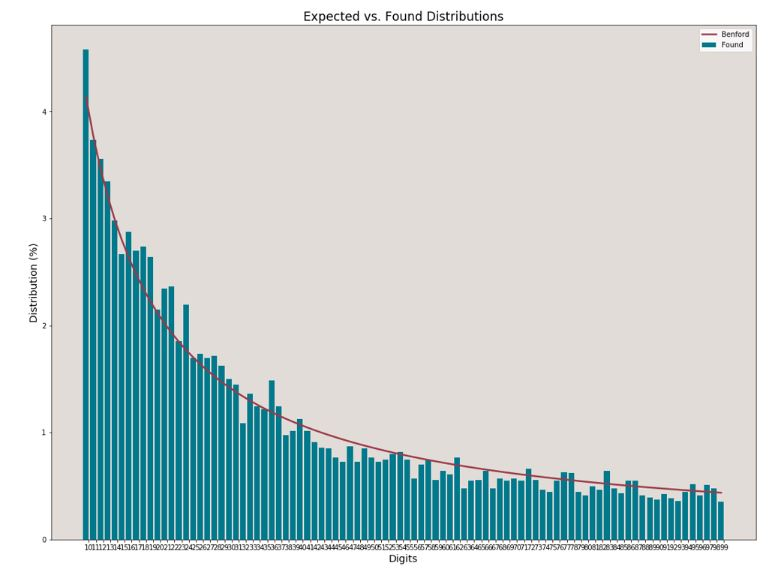
\includegraphics[width=\columnwidth]{images/benford_nsn.JPG}
  \caption{Benfords Law Verification for - NSN DS}\label{f:NSN-ds-benfordlaw}
\end{figure}

The line is Benford’s Law probabilities and the bars are 
the actual occurrences.


\subsection{Fraud Detection - Credit card transactions Dataset}
This dataset contains information on purchases made through 
the purchase card programs administered by the state and higher 
ed institutions. The purchase card information will be updated monthly 
after the end of the month. For example, July information will 
be added in August~\cite{hid-sp18-514-purchase-card-desc}

BenfordLawCSVDataSetService returned the below
output for the dataset~\cite{hid-sp18-514-purchase-card-ds}

\begin{figure}[!ht]
\centering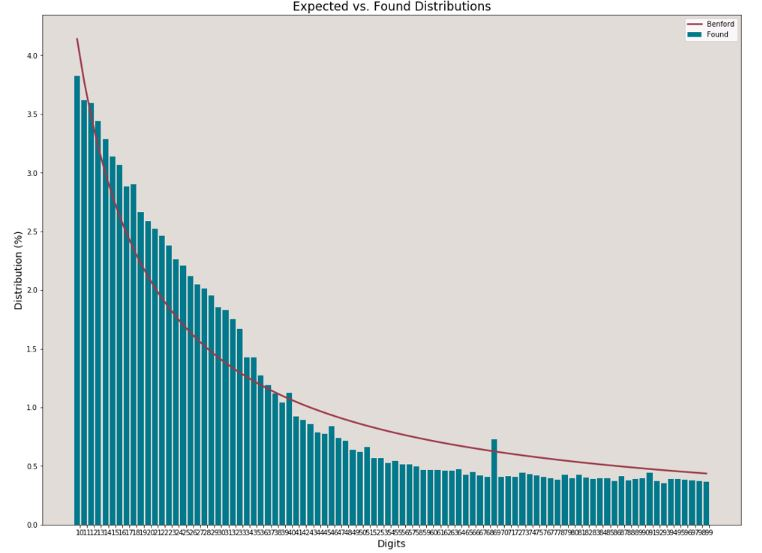
\includegraphics[width=\columnwidth]{images/ben_card_trx.JPG}
  \caption{Fraud Detection Using Benford Law}\label{f:card-ds-benfordlaw}
\end{figure}

The line is Benford’s Law probabilities and the bars are 
the actual occurrences.


\section{Conclusion}
Benford’s Law can recognize the probabilities of highly  likely or 
highly unlikely frequencies of numbers in a data set.The 
probabilities are based on mathematical logarithms of the occurrence 
of digits from the given data sets for Benford's validity. We have 
verified Benford law for stock price dataset and fraud detection on 
card transactions.The limitation with Benford Law is, it performs 
Benford Law analysis on Numeric data type column only. 
And for accurate analysis it requires large dataset.
For smaller dataset the analysis might not accurate.

As seen in the results above, the Law tends to apply the most 
to data that are uniformly distributed across several orders of magnitude. 
It may not apply if the range of values are very tight. 
The credit card transaction above is way off Benford’s 
Law prediction. This should prompt further investigation 
since credit card transactions are usually in orders of several 
magnitude. It’s either the transaction are purposely fraudulent 
or unintentionally filled with bad data or it is one 
of the few exceptions where Benford’s Law does not apply.


\bibliographystyle{ACM-Reference-Format}
\bibliography{report} 
